\documentclass{beamer}
\usetheme{Boadilla}

\usepackage{amsmath}
\usepackage{amsfonts}
\usepackage{hyperref}
\usepackage{dirtytalk}



\title{Stochastic Gradient Descent as Approximate Bayesian Inference}
\author{Skorik Sergey}
\institute{MIPT, 2022}


\begin{document}

\begin{frame}
    \titlepage
\end{frame}


\begin{frame}
    \tableofcontents
\end{frame}


\section{Continuous-Time Limit Revisited}

\begin{frame}{Problem setup}
    Consider loss functions of the following form:
    \begin{equation}\label{loss_func}
        \mathcal{L}(\theta) = \dfrac{1}{N}\sum_{n=1}^N \ell_n(\theta), \quad g(\theta) \equiv \nabla_{\theta}\mathca{L}(\theta),\,\,\, \ell_n(\theta) \equiv \ell(\theta, \boldsymbol{x}_n) \Rightarrow \mathcal{L}(\theta) \equiv \mathcal{L}(\theta, \boldsymbol{x})
    \end{equation}

    Let $\mathcal{S}$ be a set of $S$ random indices drawn uniformly at random from the set $\{1, . . . , N\}$. we call $\mathcal{S}$ a \say{minibatch} of size $S$. \\
    Then, let's define
    \begin{equation}\label{minibatch_loss_func}
        \hat{\mathcal{L}}_S(\theta) = \dfrac{1}{S}\sum_{n\in \mathcal{S}} \ell_n(\theta), \quad \hat{g}_S(\theta) \equiv \nabla_{\theta}\hat{\mathcal{L}}_S(\theta),\,\,\, g(\theta) = \mathbb{E}[\hat{g}_S(\theta)]
    \end{equation}
    We use this stochastic gradient in the SGD update
    \begin{equation}\label{SGD}
        \theta(t + 1) = \theta(t) - \varepsilon\hat{g}_S(\theta(t)), \quad \varepsilon = const
    \end{equation}
    Eqs. \ref{minibatch_loss_func} and \ref{SGD} define the discrete-time process that SGD simulates from. We will approximate it with a continuous-time process that is easier to analyze.
\end{frame}

\begin{frame}{SGD as an Ornstein-Uhlenbeck Process}
    \begin{block}{Definitions}
    Itô stochastic differential equation:
    \begin{equation}\label{ito_diff_eq}
    \begin{cases}
        dX(t) = f\left(t, X(t)\right)dt + g\left(t, X(t)\right)dW(t) \\
        X(0) = X_0
    \end{cases}
    \end{equation}
    \end{block}
    \begin{block}{Definitions}
    The Ornstein–Uhlenbeck process $X(t)$ is defined by the following stochastic differential equation:
    \begin{equation}\label{OU_process}
        dX(t) = \theta X(t)dt + \sigma dW(t)
    \end{equation}
    where $\theta > 0$, $\sigma > 0$ are parameters and $W(t)$ denotes the Wiener process.
    \end{block}
    We now show how to approximate the discrete-time Eq. \ref{SGD} with a continuous-time Ornstein-Uhlenbeck process. To justify the approximation, we make four assumptions.
\end{frame}

\begin{frame}{SGD as an Ornstein-Uhlenbeck Process}
    \begin{block}{Assumptions}
    \textbf{Assumption 1:} \textit{Observe that the stochastic gradient is a sum of $S$ independent, uniformly sampled contributions. Then, we apply the central limit theorem}
    \[\hat{g}_S(\theta(t)) = \sum_{i=1}^S \hat{g}_i(\theta(t)), \quad \hat{g}_i(\theta(t)) - i.i.d,\,\, \mathbb{E}[\hat{g}_i(\theta)] = \dfrac{1}{S}g(\theta),\, i=\overline{1, n}\]
    \[\Delta g(\theta) = \dfrac{\hat{g}_S(\theta(t)) - S\frac{1}{S}g(\theta)}{\sqrt{S}} \overset{\mathbb{P}}{\to} \mathcal{N}\left(0, \frac{1}{S}C(\theta)\right)\]
    Hence
    \begin{equation}\label{assumption_1}
        \hat{g}_S(\theta(t)) \approx g(\theta) + \dfrac{1}{\sqrt{S}}\Delta g(\theta), \quad \Delta g(\theta) \sim \mathcal{N}(0, C(\theta))
    \end{equation}
    \end{block}
\end{frame}

\begin{frame}{SGD as an Ornstein-Uhlenbeck Process}
    \begin{block}{Assumptions}
        \textbf{Assumption 2:} \textit{We assume that the covariance matrix $C(\theta)$ is approximately constant with respect to $\theta$. As a symmetric positive-semidefinite matrix, this constant matrix C factorizes as}
        \begin{equation}\label{assumption_2}
            C(\theta) \approx C = BB^{\top}
        \end{equation}
        We now define $\Delta\theta(t) = \theta(t+1) - \theta(t)$ and combine Eqs. \ref{SGD}, \ref{assumption_1} and \ref{assumption_2} to rewrite process as
        \begin{equation}\label{finite_diff_OU_proc}
            \Delta\theta(t) = -\varepsilon g(\theta(t)) + \dfrac{\varepsilon}{\sqrt{S}}B\Delta W, \quad \Delta W \sim \mathcal{N}(0, \boldsymbol{I})
        \end{equation}
        \textbf{Assumption 3:} \textit{We assume that we can approximate the finite-difference equation (\ref{finite_diff_OU_proc}) by the stochastic differential equation}
        \begin{equation}\label{assumption_3}
            d\theta(t) = -\varepsilon g(\theta(t))dt + \dfrac{\varepsilon}{\sqrt{S}}B dW(t)
        \end{equation}
    \end{block}
\end{frame}

\begin{frame}{SGD as an Ornstein-Uhlenbeck Process}
    \begin{block}{Assumptions}
        \textbf{Assumption 4:} \textit{We assume that the stationary distribution of the iterates is constrained to a region where the loss is well approximated by a quadratic function.}
        \begin{equation}\label{assumption_4}
            \mathcal{L}(\theta) = \dfrac{1}{2}\theta^{\top}A\theta
        \end{equation}
        \textit{(Without loss of generality, we assume that a minimum of the loss is at $\theta = 0$.) We also assume that $A$ is positive definite.} \\
        The four assumptions above result in a specific kind of stochastic process, the multivariate Ornstein-Uhlenbeck process. 
        \begin{equation}\label{SGD_as_OU_proc}
            d\theta(t) = -\varepsilon A\theta(t)dt + \dfrac{\varepsilon}{\sqrt{S}}B dW(t)
        \end{equation}
    \end{block}
\end{frame}

\begin{frame}{SGD as an Ornstein-Uhlenbeck Process}
    \begin{block}{Discussion}
        This connection helps us analyze properties of SGD because the Ornstein-Uhlenbeck process has an analytic stationary distribution $q(\theta)$ that is Gaussian. 
        \begin{equation}\label{stationary_OU_distribution}
            q(\theta) \propto \exp{\left(-\dfrac{1}{2}\theta^{\top}\Sigma^{-1}\theta\right)}
        \end{equation}
        The covariance $\Sigma$ satisfies
        \begin{equation}\label{Sigma_equation}
            \Sigma A + A\Sigma = \dfrac{\varepsilon}{S}BB^{\top}
        \end{equation}
        Without explicitly solving this equation, we see that the resulting covariance $\Sigma$ is proportional to the learning rate $\varepsilon$ and inversely proportional to the magnitude of $A$ and minibatch size $S$. This characterizes the stationary distribution of running SGD with a constant step size.
    \end{block}
\end{frame}

\section{SGD as Approximate Inference}

\begin{frame}{Constant Stochastic Gradient Descent}
    \begin{block}{Bayesian Inference}
      In Bayesian inference, we assume a probabilistic model $p(\theta, \boldsymbol{x})$ with data $\boldsymbol{x}$ and hidden variables $\theta$; our goal is to approximate the posterior
    \begin{equation}\label{bayesian_inference}
        p(\theta \vert \boldsymbol{x}) = \exp{\{\log p(\theta, \boldsymbol{x}) - \log p(\boldsymbol{x})\}}
    \end{equation}  
    \end{block}
    \begin{block}{Constant SGD}
        Assumption 4 says that the posterior is approximately Gaussian in the region that the stationary distribution focuses on  
        \begin{equation}\label{assump_4_posterior}
            f(\theta) \propto \exp{\{\dfrac{N}{2}\theta^{\top}A\theta\}}
        \end{equation}
        Consider a more general SGD scheme that may involve a preconditioning matrix $H$ instead of a scalar learning rate $\varepsilon$:
        \begin{equation}\label{general_SGD}
            \theta_{t+1} = \theta_{t} - H \hat{g}_S(\theta(t))
        \end{equation}
    \end{block}
\end{frame}
        
\begin{frame}{Constant Stochastic Gradient Descent} 
    \begin{block}{Constant SGD} 
        We will set the parameters of SGD to minimize the KL divergence between the stationary distribution $q(\theta)$ (Eq. \ref{stationary_OU_distribution}) and the posterior $f(\theta)$ (Eq. \ref{assump_4_posterior}).
        \begin{equation}\label{KL_minimize}
            \{H^{*}, S^*\} = \arg\min_{H, S}KL(q || f)
        \end{equation}
        Consider a scalar learning rate $\varepsilon$ (or a trivial preconditioner $H = \varepsilon\boldsymbol{I}$)
        \[KL(q || f) = -\mathbb{E}_q[\log f(\theta)] + \mathbb{E}_q[\log q(\theta)] = \] 
        \[= \dfrac{1}{2}\left(N\mathbb{E}_q[\theta^{\top}A\theta] - \log|NA| - \log|\Sigma| - D\right) = \]
        \[= \dfrac{1}{2}\left(NTr(A\Sigma) - \log|NA| - \log|\Sigma| - D\right)\]
        where $\vert \cdot \vert$ is a determinant and D -- dimension of $\theta$
    \end{block} 
\end{frame}

\begin{frame}{Constant Stochastic Gradient Descent}
    \begin{block}{Theorem 1}
         \textbf{Theorem 1 (constant SGD)} Under Assumptions A1-A4, the constant learning rate that minimizes KL divergence from the stationary distribution of constant SGD to the posterior is 
         \begin{equation}\label{theorem1}
             \varepsilon^* = 2\frac{S}{N}\frac{D}{Tr(BB^{\top})}
         \end{equation}
         \textbf{Proof:} Let $\Sigma_0 \equiv \frac{S}{\varepsilon}\Sigma$. According to eq.\ref{Sigma_equation} $\Sigma_0$ is independent with respect to $\varepsilon$.
         \[\log |\Sigma| = D \log\left(\frac{\varepsilon}{S}\right) + \log |\Sigma_0|\]
         Since $\Sigma_0$ is constant. We also need to simplify the term $Tr(A\Sigma)$
         \[Tr(A\Sigma) = \dfrac{1}{2}(Tr(A\Sigma) + Tr(\Sigma A)) = \frac{\varepsilon}{2S}Tr(BB^{\top})\]
    \end{block}
\end{frame}
         
\begin{frame}{Constant Stochastic Gradient Descent} 
    \begin{block}{Theorem 1} 
        \textbf{Proof:} The KL divergence is therefore, up to constant terms
         \begin{equation}
             KL(q||f) \overset{c}{=} \frac{\varepsilon N}{2S}Tr(BB^{\top}) - D \log\left(\frac{\varepsilon}{S}\right)
         \end{equation}
         Let $x = \frac{\varepsilon}{S}$, minimizing KL divergence over $x$ gives
         \[\frac{\partial KL(q||f)}{\partial x} = \frac{N}{2}Tr(BB^{\top}) - \frac{D}{x} = 0 \rightarrow x = \frac{2}{N}\frac{D}{Tr(BB^{\top})}\]
         After the reverse substitution, we obtain the required eq. \ref{theorem1}.
    \end{block}
\end{frame}
    
\begin{frame}{Constant Stochastic Gradient Descent}
    \begin{block}{Theorem 2}
        \textbf{Theorem 2 (Preconditioned constant SGD)} The preconditioner for constant SGD that minimizes KL divergence from the stationary distribution to the posterior is
        \begin{equation}\label{theorem2}
            H^* = \frac{2S}{N}(BB^{\top})^{-1}
        \end{equation}
        \textbf{Proof:} Ornstein-Uhlenbeck process which corresponds to preconditioned SGD according to \ref{SGD_as_OU_proc}
        \[d\theta(t) = -HA\theta(t)dt + \frac{1}{\sqrt{S}}HBdW(t)\]
        All our results carry over after substituting $ A \leftarrow HA$, $\varepsilon B \leftarrow HB$. Then
        \[\Sigma A + A\Sigma = \frac{\varepsilon}{S}BB^{\top} \rightarrow \Sigma HA + HA\Sigma = \frac{1}{S}HBB^{\top}\]
    \end{block}
\end{frame}

\begin{frame}{Constant Stochastic Gradient Descent}
    \begin{block}{Theorem 2}
        \textbf{Proof:} Eq.\ref{Sigma_equation} after the transformation and multiplication by $H^{-1}$ from the left, becomes 
        \begin{equation}\label{general_sigma_equation}
            A\Sigma + H^{-1}\Sigma A H = \frac{1}{S}BB^{\top}H
        \end{equation}
        Using the cyclic property of the trace, this implies that
        \begin{equation}\label{ASigma_Trace_general}
            Tr(A\Sigma) = \dfrac{1}{2}(Tr(A\Sigma) + Tr(H^{-1}\Sigma AH)) = \frac{1}{2S}Tr(BB^{\top}H)
        \end{equation}
        Define $Q = \Sigma H^{-1}$, hence $Q^{\top} = H^{-1}\Sigma$, since $\Sigma$, $H$ and $H^{-1}$ are symmetric. Eq.\ref{general_sigma_equation} can be written as $QA + AQ^\top = \frac{1}{S}BB^\top$. Thus, we see that $Q$ is independent of $H$. The log determinant term is up to a constant $\log |\Sigma| = \log |H| + \log |Q|$.
    \end{block}
\end{frame}

\begin{frame}{Constant Stochastic Gradient Descent}
    \begin{block}{Theorem 2}
        \textbf{Proof:} Combining Eq.\ref{ASigma_Trace_general} with this term, the KL divergence is up to a constant
        \begin{equation}
             KL(q||f) \overset{c}{=} \frac{N}{2S}Tr(BB^{\top}H) + \log |H| + \log |Q|
        \end{equation}
        Taking derivatives with respect to the entries of H results in Eq.\ref{theorem2}.
    \end{block}
    \begin{block}{Corollaries}
        In high-dimensional applications, working with large dense matrices is impractical. In those settings we can constrain the preconditioner to be diagonal. \\
        \textbf{Corollary 3:} The optimal diagonal preconditioner for SGD that minimizes KL divergence to the posterior is $H^*_{kk} = \frac{2S}{NBB^\top_{kk}}$
    \end{block}
\end{frame}

\begin{frame}{Constant SGD as Variational EM}
    Consider a supervised probabilistic model with joint distribution $p(y, \theta | x, \lambda) = p(y | x, \theta) p (\theta | \lambda)$. Our goal is to find optimal hyperparameters $\lambda$. Jointly point-estimating $\theta$ and $\lambda$ by following gradients of the log joint leads to overfitting or degenerate solutions. This can be prevented in a Bayesian approach, where we treat the parameters $\theta$ as latent variables.
    \[\lambda^* = \arg\max_{\lambda}\log p(y | x, \lambda) = \arg\max_{\lambda}\log\int_{\theta}p(y, \theta | x, \lambda)d\theta\]
    Variational expectation maximization tries to find a value for $\lambda$ that maximizes the expected log-joint probability $\mathbb{E}_q[\log(\theta, y | x, \lambda)]$ where $q(\theta)$ approximate the posterior $p(\theta | y, x, \lambda)$. \\
    Let $\mathcal{L}(\theta, \lambda) = -\log p(\theta, y | x, \lambda)$, then
    \begin{equation}\label{SGD_as_VEM}
        \theta_{t+1} = \theta_{t} - \varepsilon^* \nabla_{\theta}\mathcal{L}(\theta_t, \lambda_t), \quad \lambda_{t+1} = \lambda_{t} - \rho_t\nabla_{\lambda}\mathcal{L}(\theta_t, \lambda_t)
    \end{equation}
    The $\lambda$ update uses a decreasing learning rate $\rho_t$ and therefore converges to a local optimum.
\end{frame}

\begin{frame}{Stochastic Gradient with Momentum}
    The updates of SGD with momentum are
    \[\begin{cases}
        v(t+1) = (1 - \mu)v(t) - \varepsilon\hat{g}_S(\theta(t)) \\
        \theta(t + 1) = \theta(t) + v(t+1) \\
    \end{cases}\]
    As before we assume a quadratic objective $\mathcal{L} = \frac{1}{2}\theta^\top A \theta$. Going through the same steps A1-A4, we find
    \begin{equation}\label{OU_proc_SGD_momentum}
        \begin{cases}
            dv = -\mu vdt - \varepsilon A \theta dt + \frac{1}{\sqrt{S}}\varepsilon B dW \\
            d\theta = v dt \\
        \end{cases}
    \end{equation}
    We solve this set of stochastic equations asymptotically for the long-time limit. 
    \[d\mathbb{E}[v] = -\mu\mathbb{E}[v]dt - \varepsilon A \mathbb{E}[\theta]dt, \quad d\mathbb{E}[\theta] = \mathbb{E}[v]dt\]
\end{frame}

\begin{frame}{Stochastic Gradient with Momentum}
    In order to compute the stationary distribution, we derive and solve similar equations for the second moments. We derive the following conditions:
    \begin{equation}
    \begin{split}
        \mathbb{E}[vv^\top] = \frac{\varepsilon}{2}\mathbb{E}[\theta\theta^\top]A + \frac{\varepsilon}{2}A\mathbb{E}[\theta\theta^\top], \\
        \mu\mathbb{E}[vv^\top] = \frac{\varepsilon^2}{2S}BB^\top
    \end{split}
    \end{equation}
    $\mathbb{E}[vv^\top]$  is a matrix of expected kinetic energies, while $\frac{1}{2}(\mathbb{E}[\theta\theta^\top]A + A\mathbb{E}[\theta\theta^\top])$ has the interpretation of a matrix of expected potential energies. The first equation is the conservation of energy in an equilibrium system. The second equation can be interpreted as the fluctuation-dissipation theorem.  Combining both equations and using $\Sigma = \mathbb{E}[vv^\top]$ yields
    \begin{equation}\label{momentum_sigma_equation}
        \Sigma A + A\Sigma = \frac{\varepsilon}{\mu S}BB^\top
    \end{equation}
    This is exactly Eq.\ref{Sigma_equation} of SGD without momentum. 
\end{frame}

\begin{frame}{Stochastic Gradient with Momentum}
    \begin{block}{Discussion}
        The Eq.\ref{momentum_sigma_equation} is exactly Eq.\ref{Sigma_equation} with the difference that the noise covariance is re-scaled by a factor $\frac{\varepsilon}{\mu S}$ instead of $\frac{\varepsilon}{S}$. \\
        Only the combination $\frac{\varepsilon}{\mu S}$ affects the KL divergence to the posterior. Thus, no single optimal constant learning rate exists—many combinations of $\varepsilon$, $\mu$, and $S$ can yield the same stationary distribution. But different choices of these parameters will affect the dynamics of the Markov chain. For example, Sutskever et al. (2013) observe that, for a given effective learning rate $\frac{\varepsilon}{\mu S}$ using a smaller $\mu$ sometimes makes the discretized dynamics of SGD more stable. Also, using very small values of µ while holding $\frac{\varepsilon}{\mu}$ fixed will eventually increase the autocorrelation time of the Markov chain. 
    \end{block}
\end{frame}

\section{Discussion}

\begin{frame}{Discussion}
    \begin{block}{Estimating noise covariance}
        In order to use our theoretical insights in practice, we need to estimate the stochastic gradient noise covariance $C \equiv BB^\top$. We do this in an online manner. Let $g_t$ be the full gradient, $\hat{g}_{S,t}$ be the stochastic gradient of the full minibatch and $\hat{g}_{1,t}$ be the stochastic gradient of the first sample in the minibatch at time $t$. For large $S$ we can approximate $g_t \approx \hat{g}_{S,t}$ and thus obtain an estimator of the noise covariance by $(\hat{g}_{1,t} - \hat{g}_{S,t})(\hat{g}_{1,t} - \hat{g}_{S,t})^\top$ we can now build an online estimate $C_t$ that approaches $C$ by the following recursion
        \begin{equation}\label{covariance_estimation}
            C_t = (1 - \kappa_t)C_{t-1} + \kappa_t(\hat{g}_{1,t} - \hat{g}_{S,t})(\hat{g}_{1,t} - \hat{g}_{S,t})^\top
        \end{equation}
        $\kappa_t$ is a decreasing learning rate. Ahn et al. (2012) have proven that such an online average converges to the noise covariance in the optimum at long times  (provided that $\kappa_t \sim \frac{1}{t}$ and that $N$ is sufficiently large).
    \end{block}
\end{frame}

\begin{frame}{Discussion}
    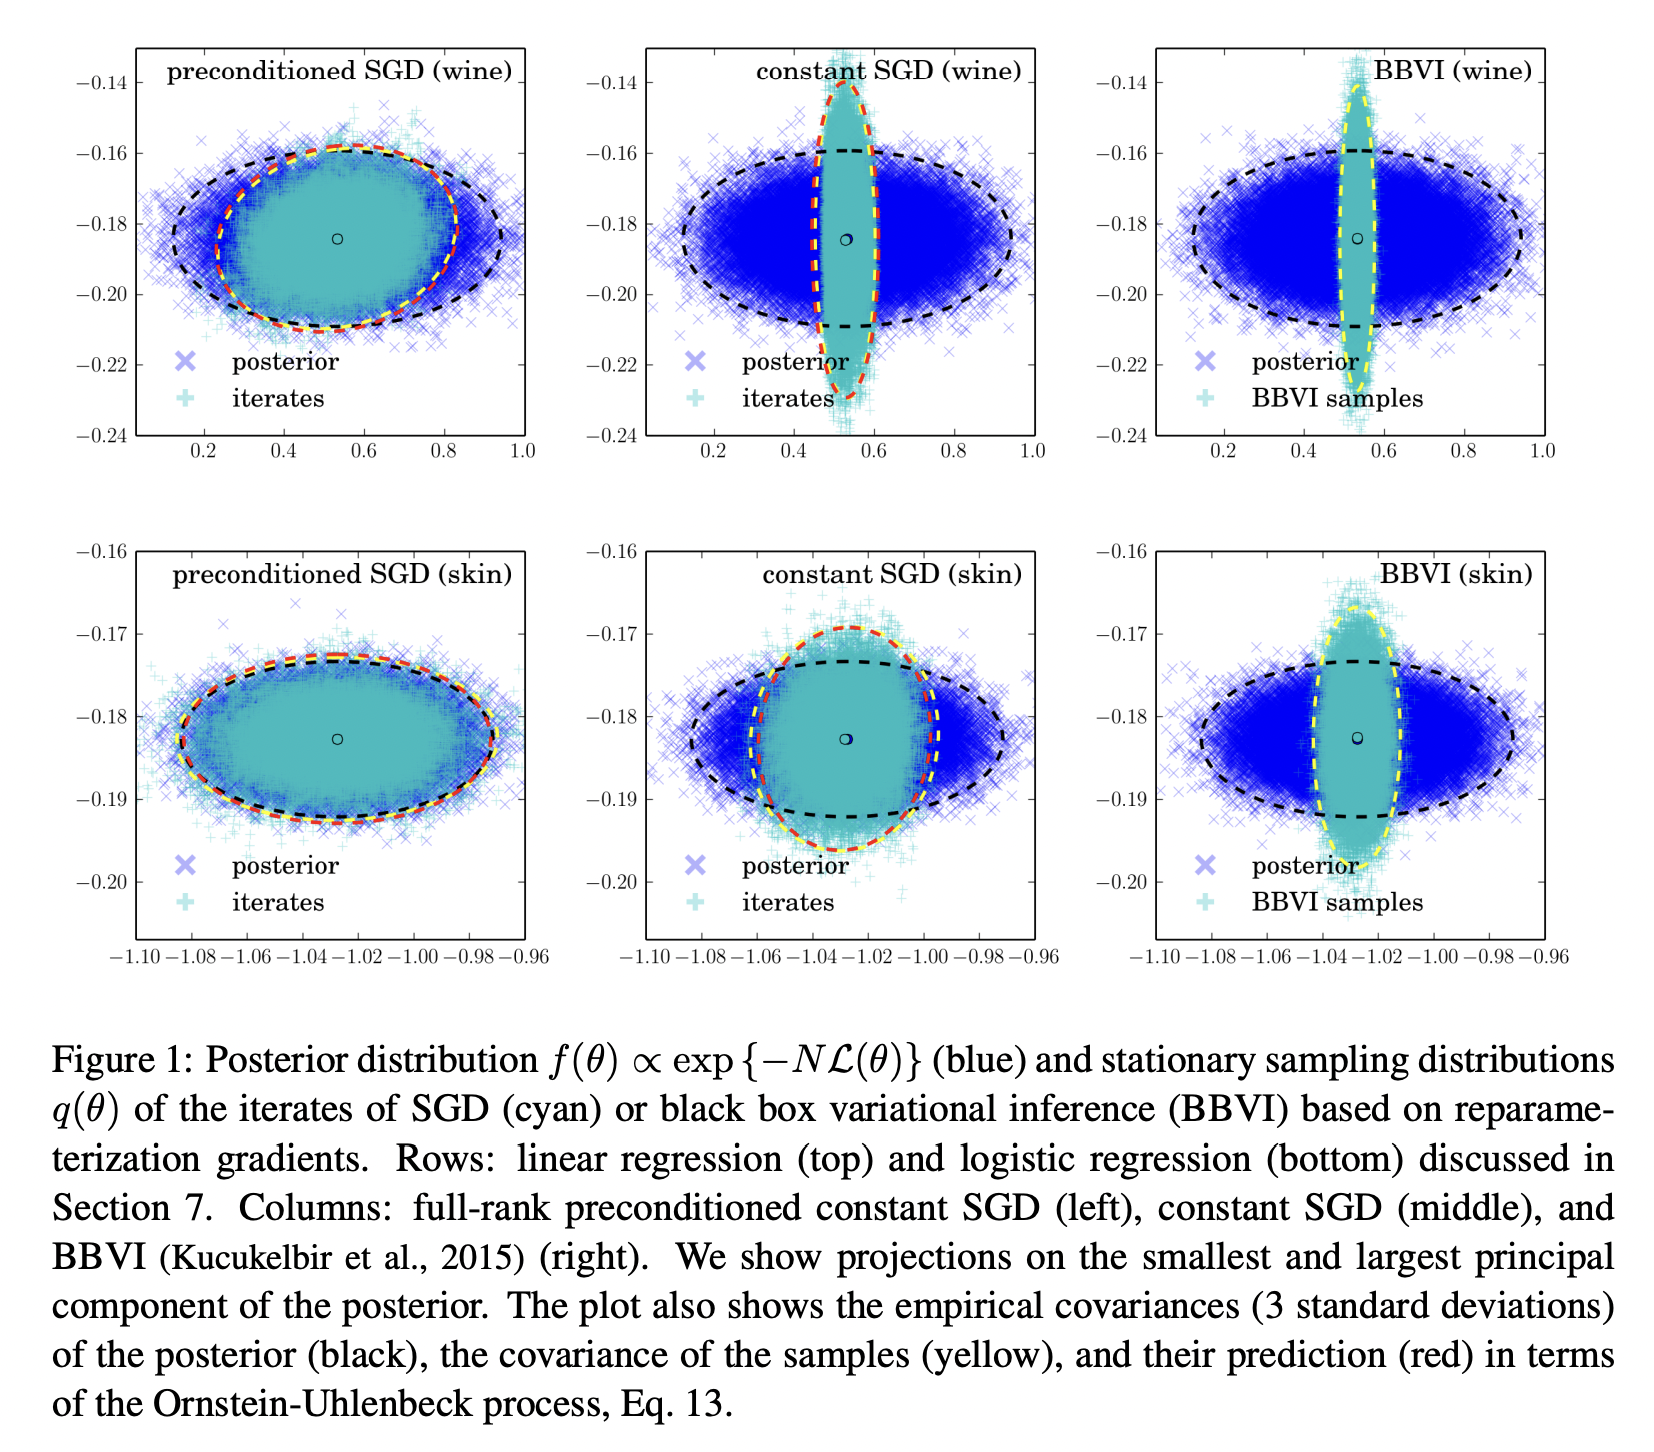
\includegraphics[width=10cm, height=8cm]{fig1.png}
\end{frame}

\begin{frame}{Discussion}
    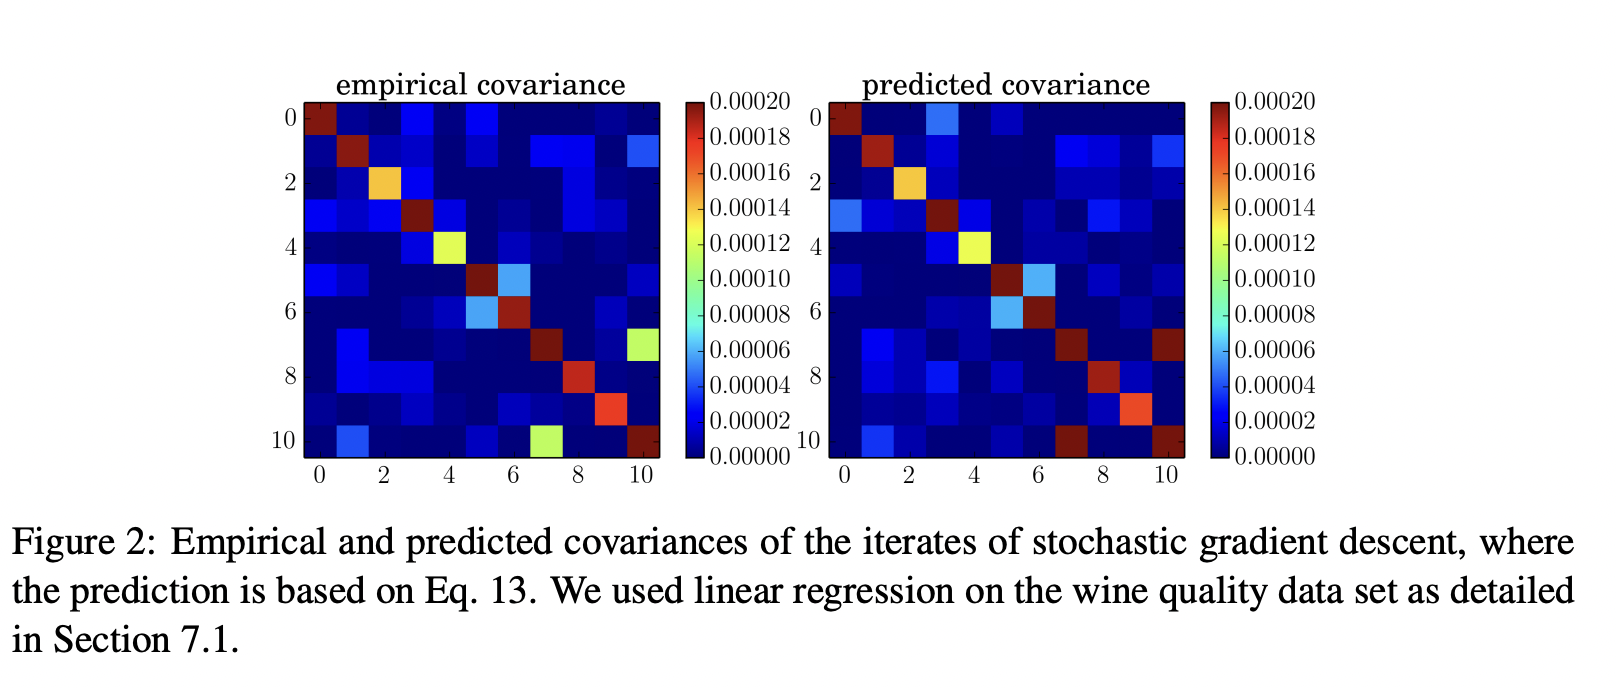
\includegraphics[width=10cm, height=6cm]{fig2.png}
    
\end{frame}
\end{document}
